    
    \section{Some Bridge related topics}
    \subsection{Finding Bridges}
    Just check if the lowest back edge of the bottom most vertex off an edge in a dfs tree entered in a time later than the time the top most vertex entered the dfs.
    \inputwithhash{./solutions/Graph/bridges.cpp}
    
    \subsection{Articulation Points}
    Vertexs which when increase the number of components. The main idea is the same of finding bridges, utilize the low to check things in the dfs tree.
    \inputwithhash{./solutions/Graph/articulation.cpp}

    \subsection{Block Cut Tree}
    \begin{center}
        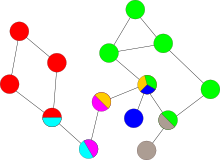
\includegraphics[]{imgs/bicomp.png}
    \end{center}
    Construct a tree of bi-connected components of the graph. Some of the approaches related to this structure needs you to do some updates in the parent of the node.

    The application is a problem with a lot of queries each query will give 3 vertices $a$,$b$ and $c$ and ask if there is a path that goes from $a$ to $b$, without passing in $c$. The answer is no if $a  == b$, $a == c$ or $c$ is an articulation point and is in the path of the block cut tree going from $a$ to $b$. The build is $\mathcal{O}(N)$, it gives you a tree, and you what you want from it.
    \inputwithhash{./solutions/Graph/block_cut_tree.cpp}

    \subsection{Two Edge Connected Components}
    Decompose the graph in Components connected by at least two edges. Can be used to create a tree as well, a "block cut" decomposition, but with edges instead of vertices.

    \inputwithhash{./solutions/Graph/2cc.cpp}
